\documentclass[]{article}
\usepackage{graphicx}
\newcommand*{\affaddr}[1]{#1}
\newcommand*{\affmark}[1][*]{\textsuperscript{#1}}
\usepackage{listings} 
\usepackage{xcolor}
\lstset{
	language=Python,  
	frame=shadowbox, %把代码用带有阴影的框圈起来
	rulesepcolor=\color{red!20!green!20!blue!20},%代码块边框为淡青色
	keywordstyle=\color{blue!90}\bfseries, %代码关键字的颜色为蓝色,粗体
	commentstyle=\color{red!20!green!90}\textit,    % 设置代码注释的颜色
	showstringspaces=false,%不显示代码字符串中间的空格标记
	numbers=left, % 显示行号
	numberstyle=\tiny,    % 行号字体
	stringstyle=\ttfamily, % 代码字符串的特殊格式
	breaklines=true, %对过长的代码自动换行
	extendedchars=false,  %解决代码跨页时,章节标题,页眉等汉字不显示的问题
	texcl=true}
\begin{document}
\title{ENGN4528 Computer Vision – 2021 Computer-Lab 2 (C-Lab2)}

\author{Hongxiang Zhang(u7101924)\\
	\affaddr{\affmark[1]Australian National University}
}


\maketitle
%
\section{Tasks Harris Corner Detector}
\subsection{Read and understand the above corner detection code (page 3). Note that we have separated code in different parts/blocks (which could be referred easily by its block number in later questions.)}
For the first block, it imports the NumPy. The second block defines a convolution operation that inputs the image and a kernel, then outputs the image matrix after convolution. The third part defines a function that returns a Gaussian kernel with sigma equal to 0.5. The fourth block, dx,dy are two soble kernels that are used to calculate the gradient of the image corresponding to the x-axis and y-axis. The fifth block is to get a Gaussian kernel from the $fspecial$ function. The sixth block is using the Gaussian kernel to smooth the gradient matrix which is x-axis, y-axis, and xy-axis.
\subsection{Complete the missing parts, rewrite them to ‘harris.py’ as a python script, and design appropriate function signature (1 mark).}
In block 7, What we need to do is calculate R-value for each pixel, and perform thresholding and non-maximum suppression. First, we generate a covariance matrix of the gradient for each pixel, using the harris matrix to calculate R-value, also, find the max R-value. Second, using 0.02*Rmax as the threshold to find the pixel that R-value is greater than the threshold. Third, perform the non-maximum suppression to the result. The output is the coordinate of the corner point.

\subsection{Comment on the codes in every line of your solution in block \#7 (0.5 mark).}
\begin{lstlisting}
# Task: Compute the Harris Cornerness
#
height,width = bw.shape
result,R,Rmax = np.zeros((height,width)),np.zeros((height,width)),0 # init R matrix, result matrix which record where the corner is, init Rmax as 0

for i in range(height):
	for j in range(width):
		M = np.zeros((2,2))
		M[0,0],M[0,1],M[1,0],M[1,1]=Ix2[i,j],Ixy[i,j],Ixy[i,j],Iy2[i,j] # For each pixel init the Covariance matrix of gradient
		R[i,j] = np.linalg.det(M) - k*(np.dot(np.trace(M),np.trace(M))) # using harris matrix to calculate the R value
		if R[i,j]>Rmax:
			Rmax = R[i,j] # find the max R value
# Task: Perform non-maximum suppression and
#       thresholding, return the N corner points
#       as an Nx2 matrix of x and y coordinates
#
#  compare whith threshold
count = 0;
for i in range(2,height-2):
	for j in range(2,width-2):
		if R[i,j] > 0.02*Rmax: # using Rmax*0.02 as threshold
			result[i,j] = 1
			count = count +1
print(count)
for i in range(2,height-2):
	for j in range(2,width-2):
		if result[i,j]==1:
			tmp = R[i-1:i+1,j-1:j+1]
			if R[i,j]!=tmp.max(): # perform non-maximum suppression
				result[i,j]=0
				count-=1

x,y =[],[]
for i in range(height):
	for j in range(width):
		if result[i,j]==1:
			x.append(i)
			y.append(j)
\end{lstlisting}

\subsection{Test this function on the provided four test images (Harris-[1,2,3,4].jpg, they can be downloaded from Wattle). Display your results by marking the detected corners on the input images (using circles or crosses, etc)}
Show on .py file.
Answer:\\
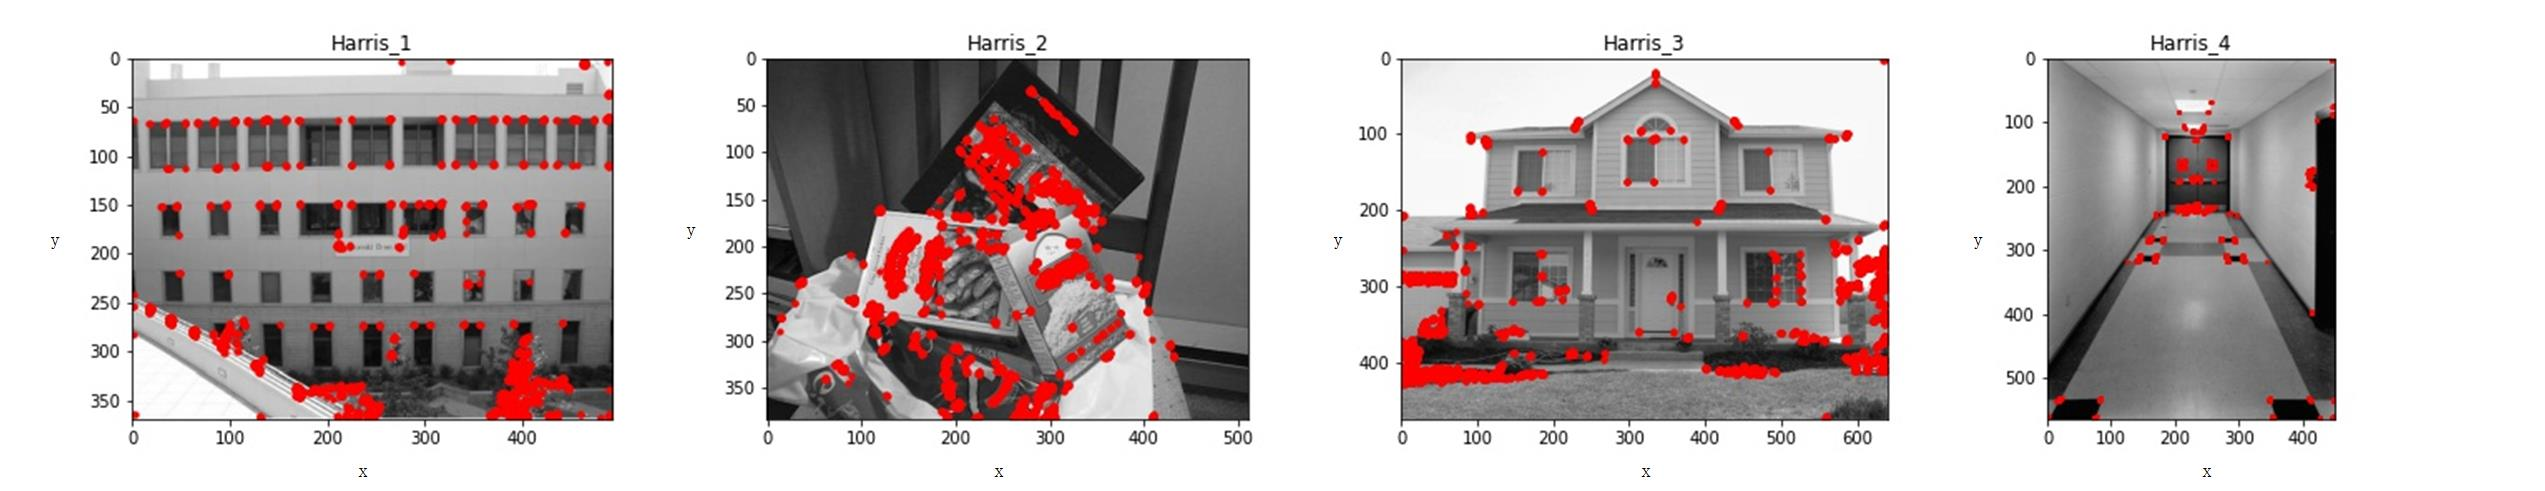
\includegraphics[width=15cm]{fig1.jpg}

\subsection{Compare your results with that from python’s built-in function cv2.cornerHarris() (0.5 mark), and discuss the factors that affect the performance of Harris corner detection (1 mark).}
Answer:\\
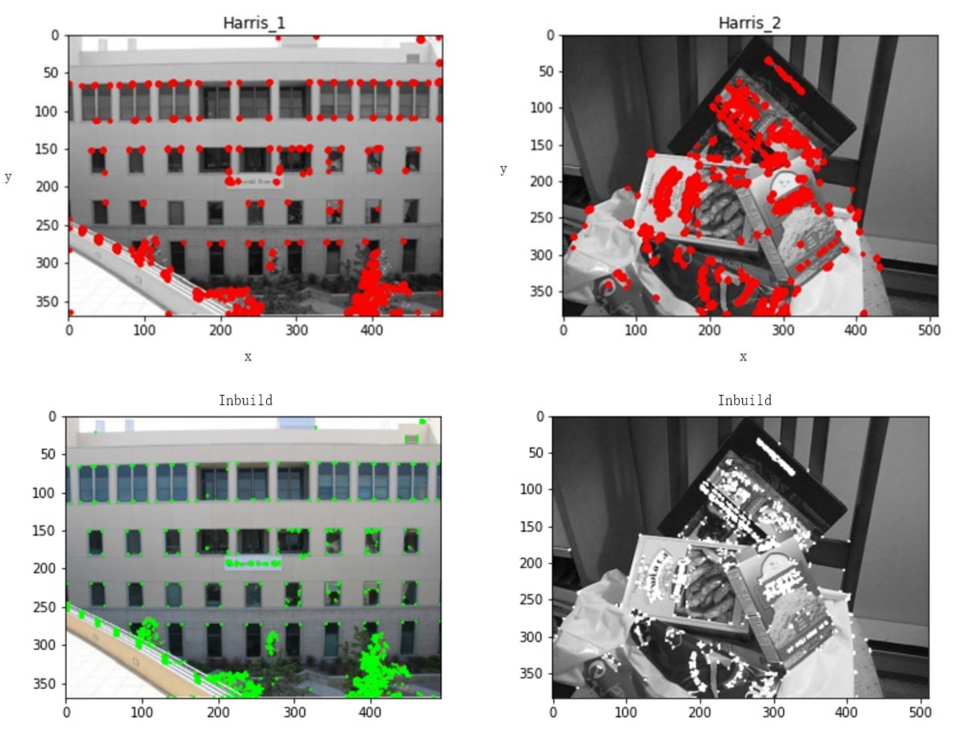
\includegraphics[width=12cm]{fig2.png}\\
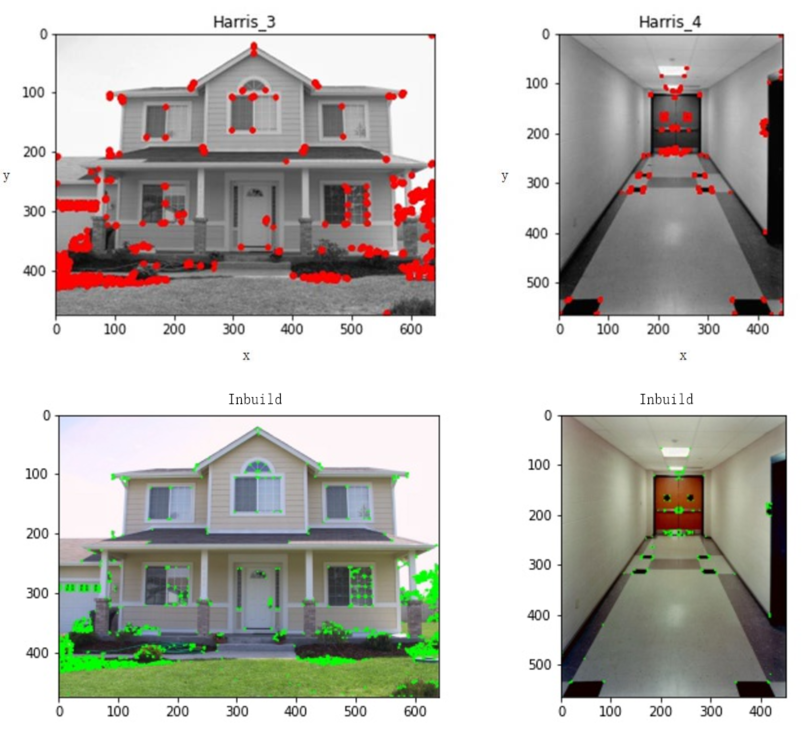
\includegraphics[width=12cm]{fig3.png}

threshold, kernel size, k can affect the performance of Harris corner recognization. The greater threshold can eliminate more points, which means fewer corner points can be detected. kernel size affects the result of convolution results.

\subsection{Test this function on ‘Harris-5.jpg’ (Harris-5.jpg can be downloaded from wattle.). Analyse the results why we cannot get corners by discussing and visualising your corner response scores of the image. (0.5 mark)}
Answer: Because there is no corner in this graph, and we ignore the corner point which located on the edge of the image.\\
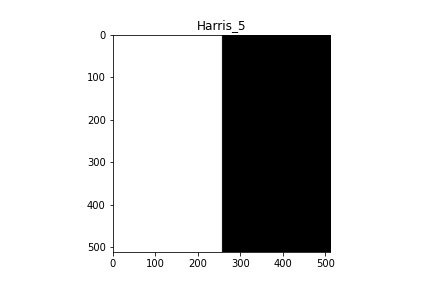
\includegraphics[width=10cm]{Harris_5_.jpg}
\subsection{Test this function on ‘Harris-6.jpg’ (Harris-6.jpg can be downloaded from wattle.).
	Plot your harris corner detector results in your report and propose a solution to obtain the salient corners which is robust to noise. (0.5mark)}
Answer: In the first graph, It detects a corner point located in the straight line. In this case, we choose another threshold to limit the corner point. As shown in the second graph, we got a salient corner point image.\\
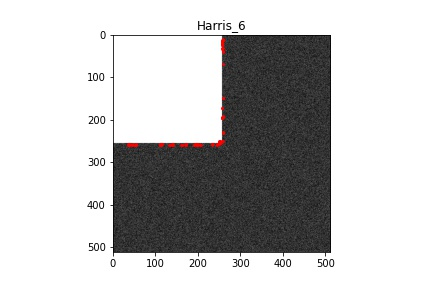
\includegraphics[width=7cm]{Harris_6_.jpg}
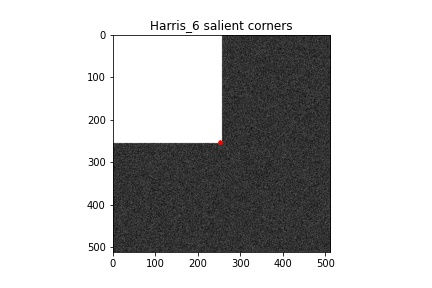
\includegraphics[width=7cm]{Harris_6salient.jpg}


\section{K-Means Clustering and Color Image Segmentation}
\subsection{Implement your own K-means function my\_kmeans().The input is the data points to be processed and the number of clusters, and the output is several clusters of your data (you can use a cell array for clusters). Make sure each step in K-means is correct and clear, and comment on key code fragments (1.5 marks).}
For k-means, we first init the clusters randomly. Then using the distance of pixel and cluster to calculate each pixel which clusters it belongs to. After that, we update the center of each cluster using the pixels that belong to the corresponding cluster.\\
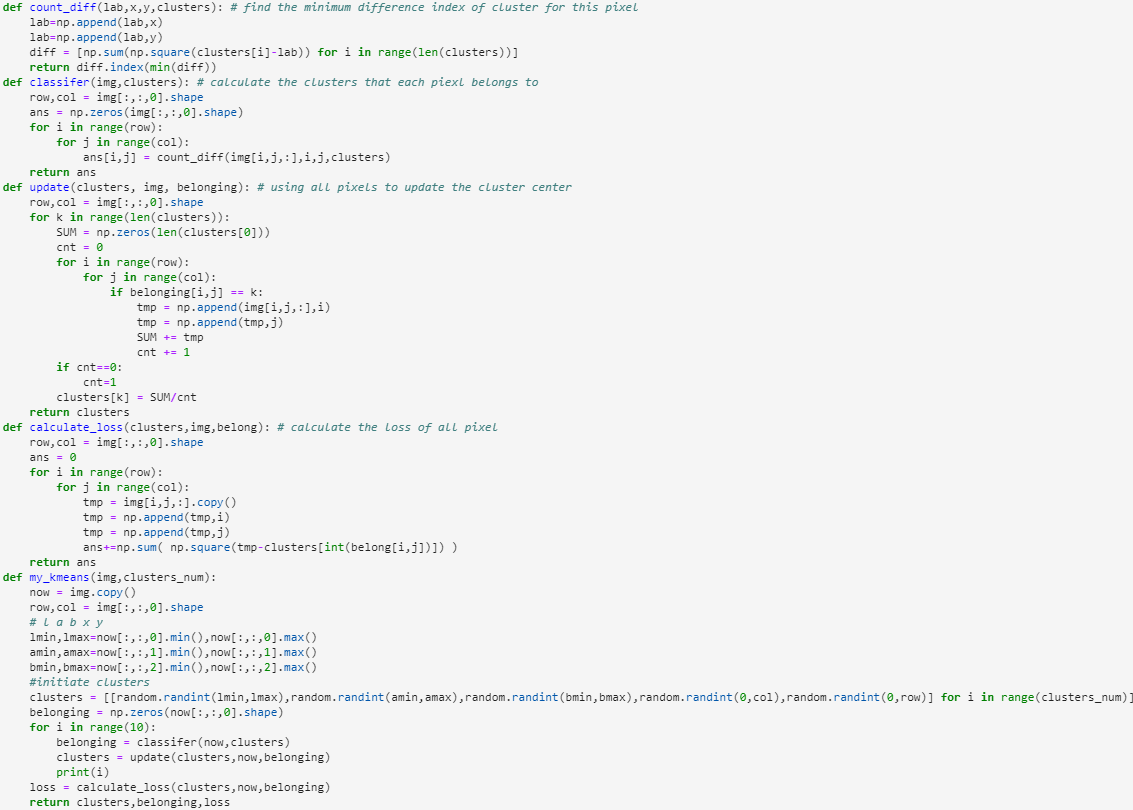
\includegraphics[width=15cm]{code.png}
\subsection{Apply your K-means function to color image segmentation.}
\subsubsection{using different numbers of clusters}
Answer: We choose clusters with number 38, 40, 42 and 44. And we found clusters with 42 has the best performace.\\

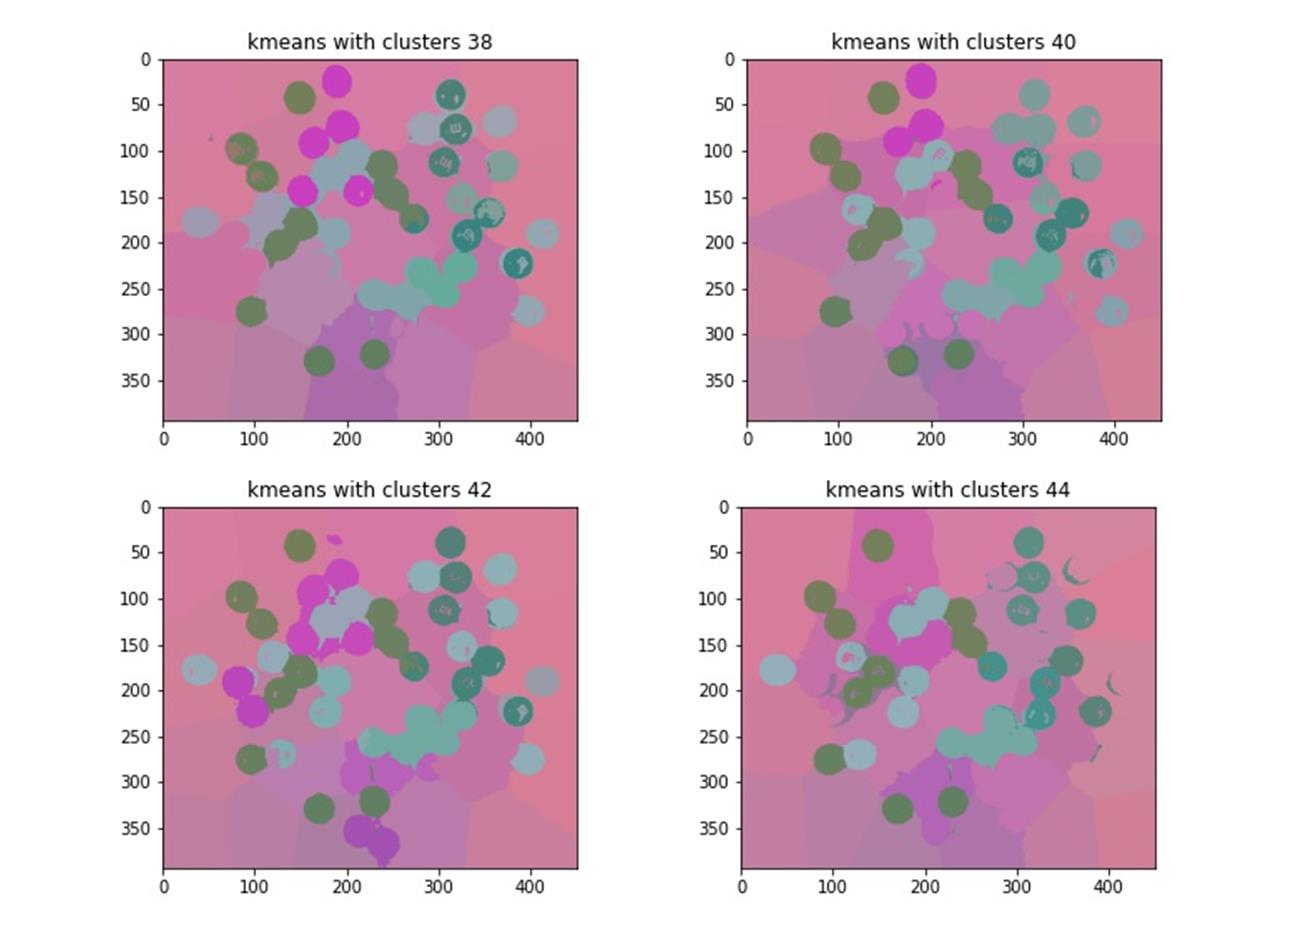
\includegraphics[width=13.5cm]{clusters.jpg}\\
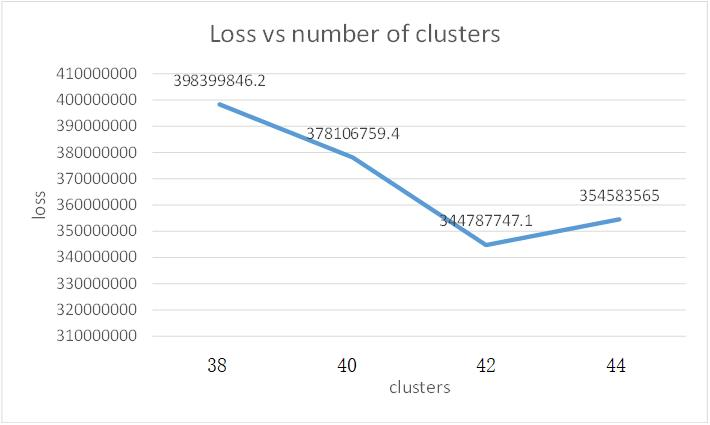
\includegraphics[width=10cm]{loss1.jpg}


\subsubsection{and with and without pixel coordinates}
Answer: We choose 7 clusters to compare the result that with and without pixel coordinates. choosing the same number of clusters, model without coordinates performe better.\\

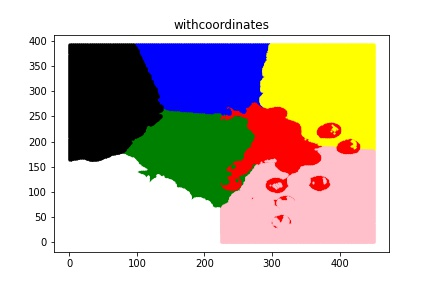
\includegraphics[width=7cm]{with_coordinates.jpg}
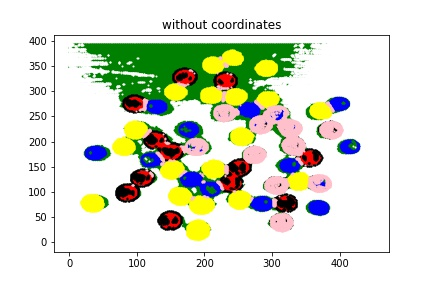
\includegraphics[width=7cm]{without_coordinates.jpg}

\subsection{The standard K-means algorithm is sensitive to initialization (e.g. initial cluster centres/seeds). One possible solution is to use K-means++, in which the initial seeds are forced to be far away from each other (to avoid local minimum). Please read the material http://ilpubs.stanford.edu:8090/778/1/2006-13.pdf, summarize the key steps in the report (0.5 mark), and then implement K-means++ in your standard algorithm as a new initialization strategy (0.5 mark). Compare the image segmentation performance (e.g., in terms of convergence speed and segmentation results [by plotting the segmentation results in the report]) of this new strategy, with that of standard K-means, using different numbers of clusters and the same 5-D point representation, *namely [ L, a*, b*, x, y,] ( L, a, b , pixel coordinates)* as that from previous question (0.5 mark).}
For k-means++, Let $D(x)$ denote the shortest distance of a data point to the cluster.

1. Arbitrarily choose an initial centers $c_1$ from $X$ which is the data points set.

2. Take a new center $c_i$, choosing $x_j\in X$ with probility $P(j)=\frac{D(x_j)^2}{\sum_{x_j\in X}^{}D(x_j)^2}$.

3. Repeat step 2, until have k centers.

4. For each $i\in \{1,...,k\}$, set the cluster $C_i$ to be the set of points in $X$ that are closer to $c_i$ than thay are to $c_j$ for all $j\neq i$

5. For each $i\in \{1,...,k\}$, set $c_i$ to be the center of mass of all points in $C_i: c_i = \frac{1}{|C_i|}\sum_{x\in C_i}^{x}$

6. Repeat Step 3,4 untiln clusters not changes.
\\ \hspace*{\fill} \\
K-means++ are implement in the code file.

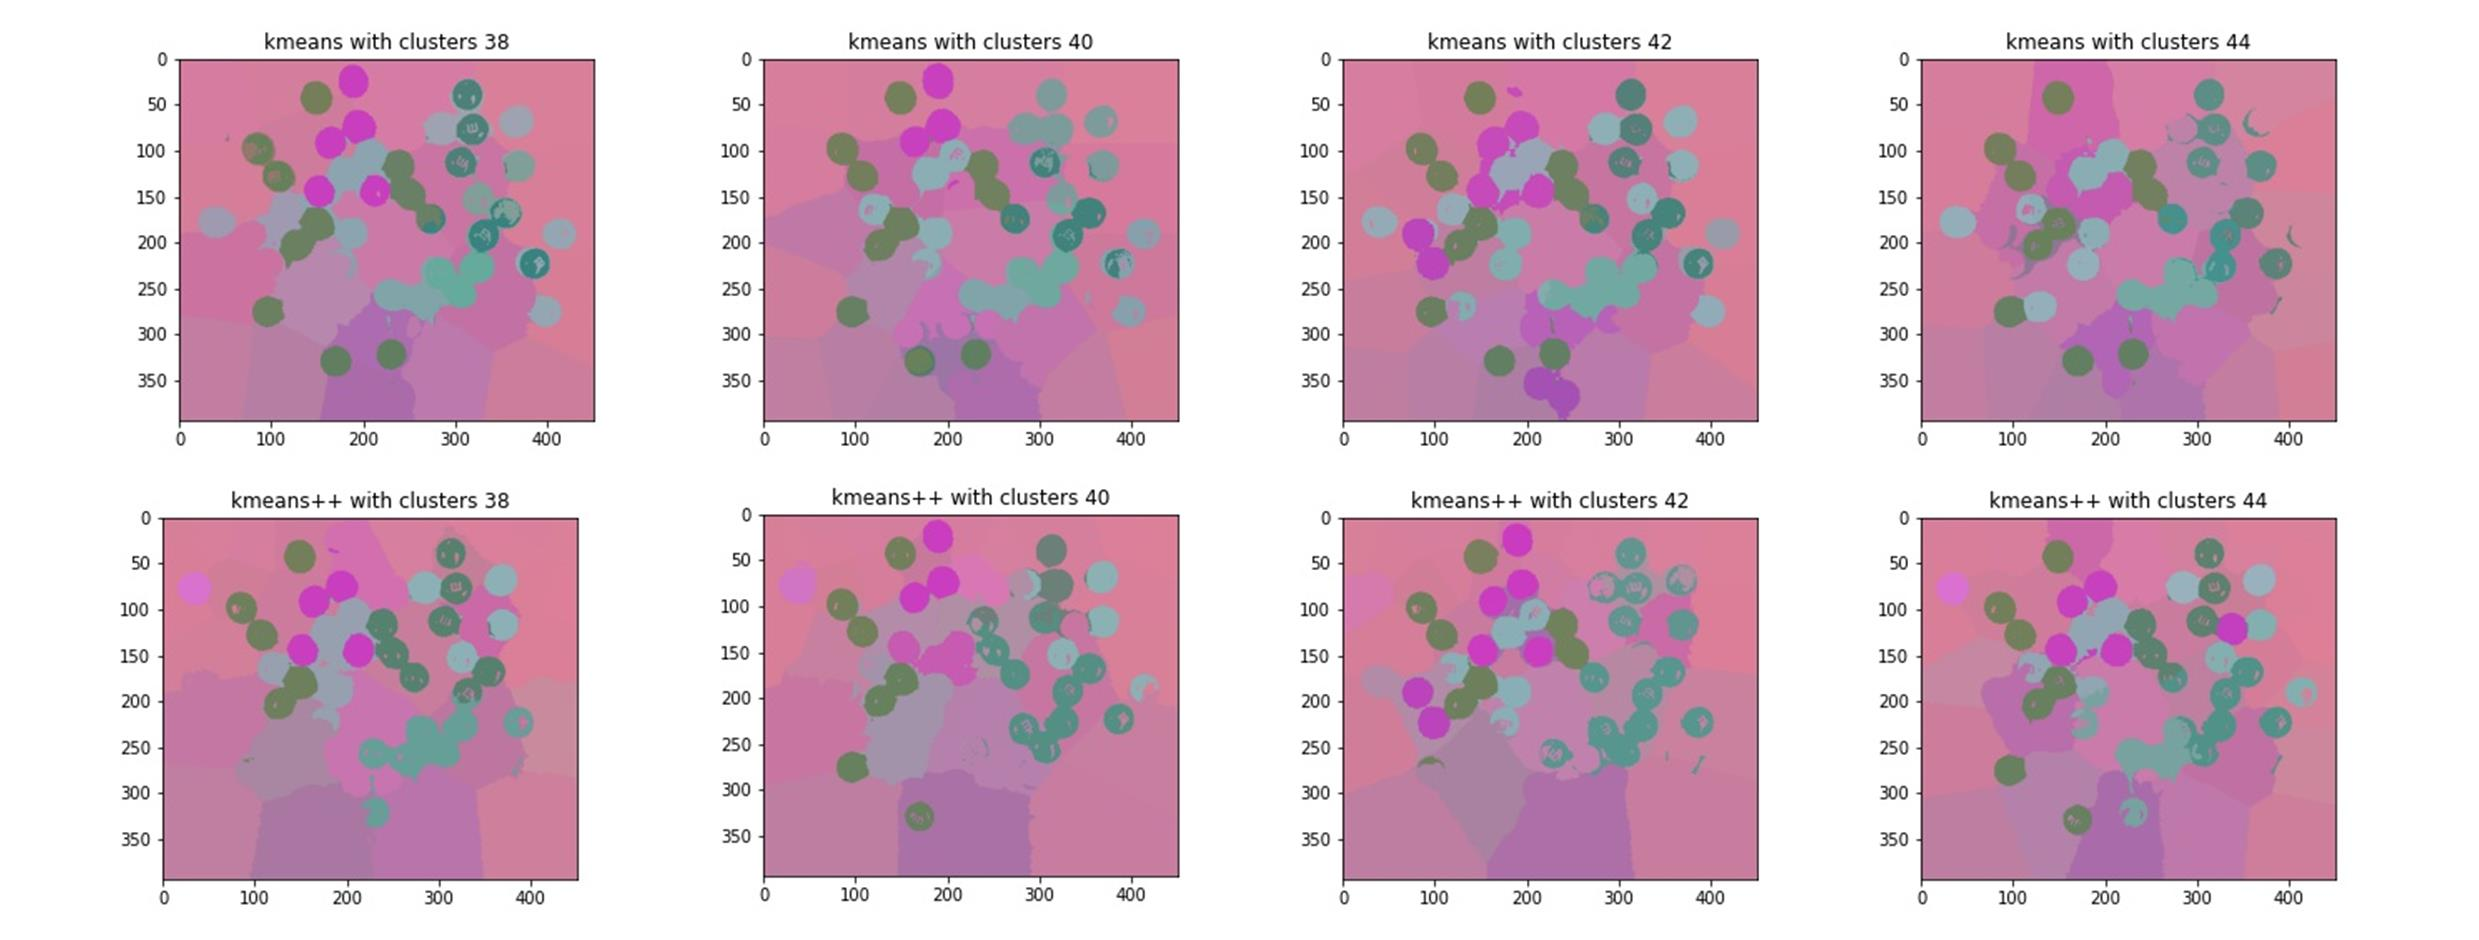
\includegraphics[width=15cm]{kmeansvsplus.jpg}
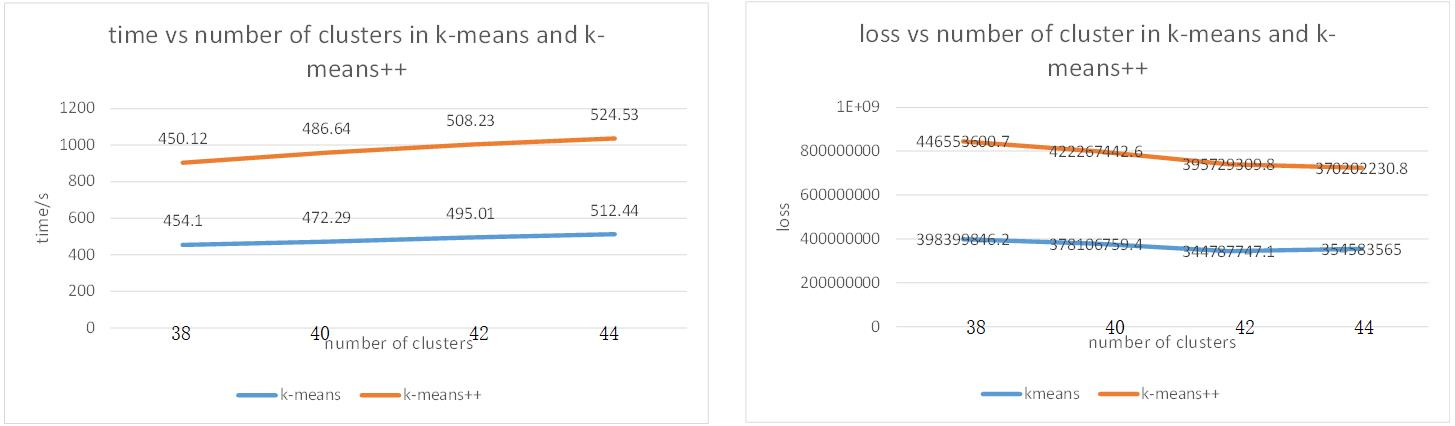
\includegraphics[width=15cm]{timeloss.jpg}
After compareation, we found kmeans++ need more time than k-means, and when classify a large number of data, it may have a worse performance than k-means, because the theory of k-means++ is random choosing clusters .

\section{Face Recognition using Eigenface.}
\subsection{Please unzip the face images and get an idea what they look like. Then please take 10 different frontal face images of yourself, convert them to grayscale, and align and resize them to match the images in Yale-Face. Explain why alignment is necessary for Eigen-face (0.5 mark).}
Because PCA transforms the original data into a set of linearly independent representations of each dimension through a linear transformation which is used to extract the main feature vector and reduce dimensions. It is hard to extract the main feature vector and reduce dimensions without alignment.

\subsection{Train an Eigen-face recognition system. Specifically, at least your face recognition system should be able to complete the following tasks:}
\subsubsection{Read all the 135 training images from Yale-Face, represent each image as a single data point in a high dimensional space and collect all the data points into a big data matrix.}
\subsubsection{Perform PCA on the data matrix (1 mark), and display the mean face (1 mark). Given the size and the large number of input images, directly performing eigen value decomposition of the covariance matrix would be slow. Please read lecture notes and find a faster way to compute eigen values and vectors, explain the reason (1 mark) and implement it in your own code (1 mark).}
Answer:\\
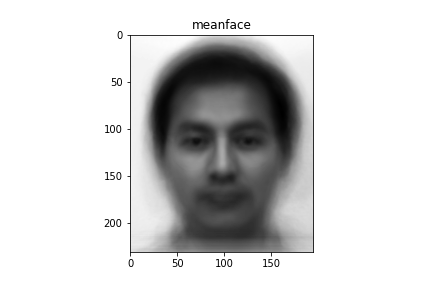
\includegraphics[width=7cm]{meanface.png}

All data were stored in a matrix $X$ with shape(42000,135). 135 represents the number of images. To calculate the eigen values and vectors, we need to calculate the covariance matrix first. There are two ways to get covariance matrix, which is $X.T@X$ shaped (135,135) and $X@X.T$ shaped (4000,4000). In this task, we choose $X.T@X$ which has lower dimensions and can calculate faster. It represents the covariance of each image.

Details are implement in code.
\subsubsection{Determine the top k principal components and visualize the top-k eigenfaces in your report (1 mark). You can choose k=10 or k=15.}
Answer: In this task, we use 15 as k.\\
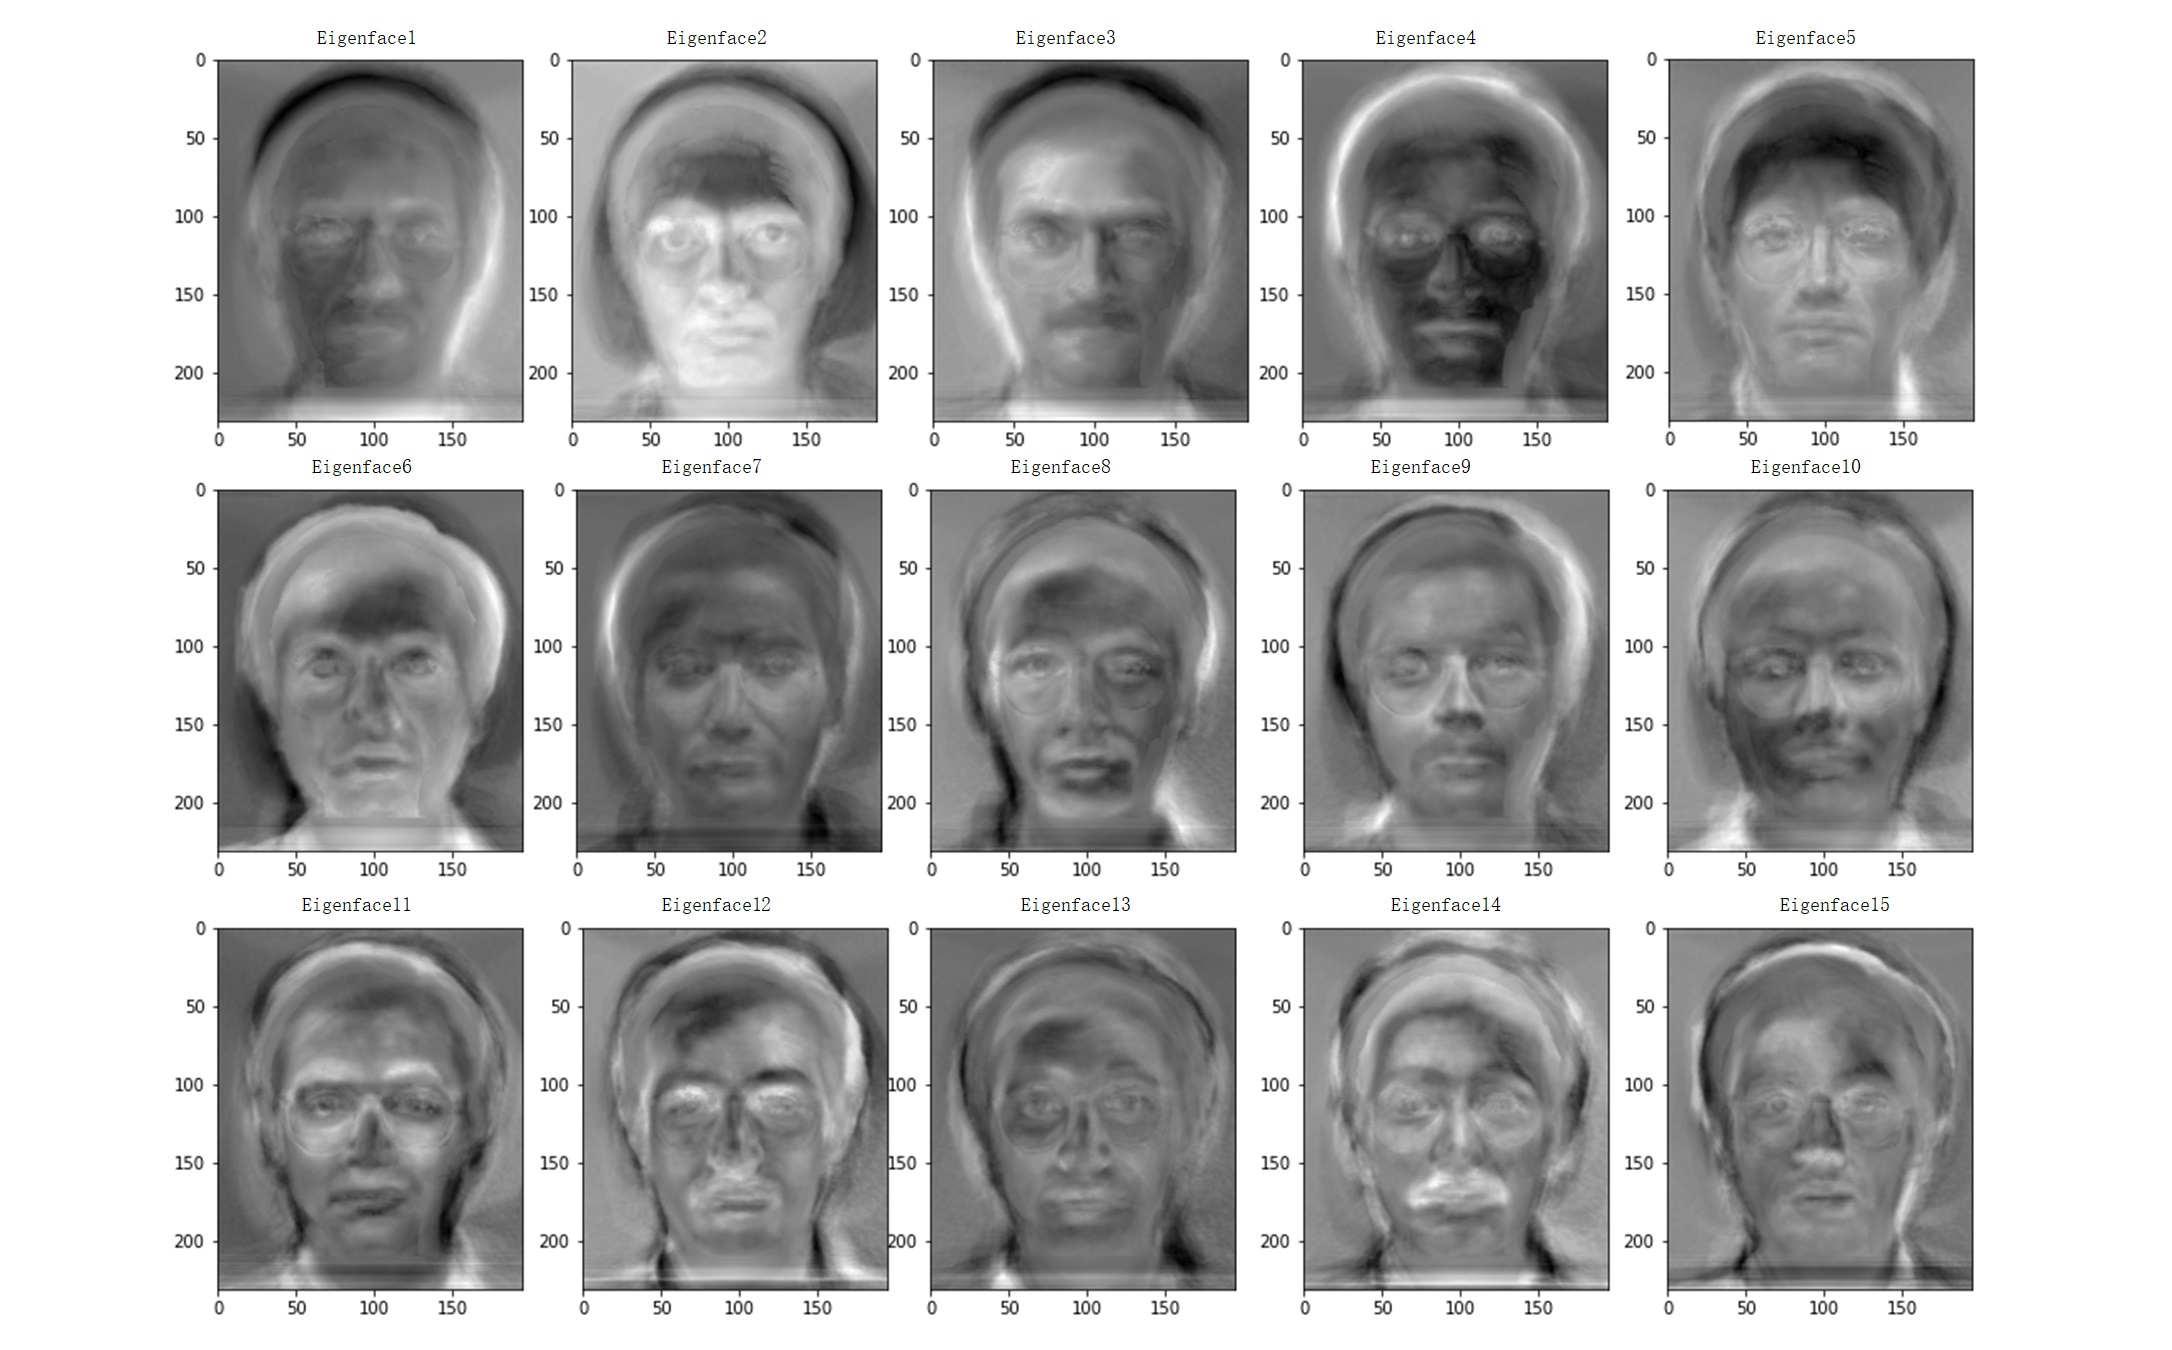
\includegraphics[width=15cm]{eigenfaces.jpg}

\subsubsection{For each of the 10 test images in the Yale-Face dataset, please read in an image as the reference one, and determine its projection onto the basis spanned by the top k eigenfaces. Use this projection as feature to perform a nearest-neighbour search over all 135 faces, and find out the top three face images that are most similar to the reference one. Show these top 3 faces next to the test image in your report (1.5 marks). Please report and analyze the recognition accuracy of your method (1 mark).}
Answers: The  accuracy is 100\%. We choose 15 as k, because we found there are 15 people in the training set, which means there are 15 eigenfaces in this task. I think that is the main reason why our accuracy is high.\\
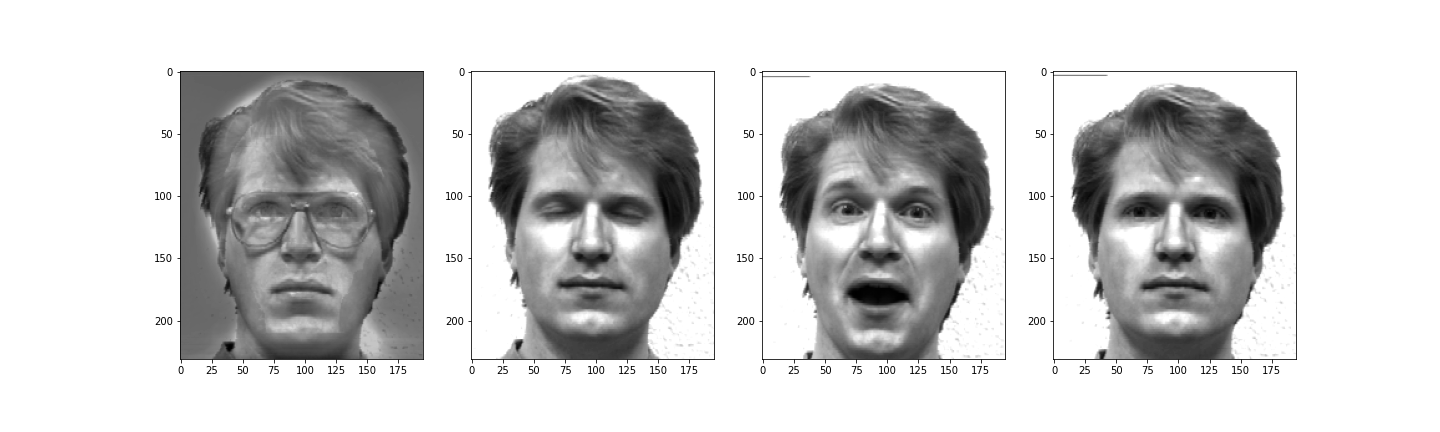
\includegraphics[width=15cm]{1top3.png}
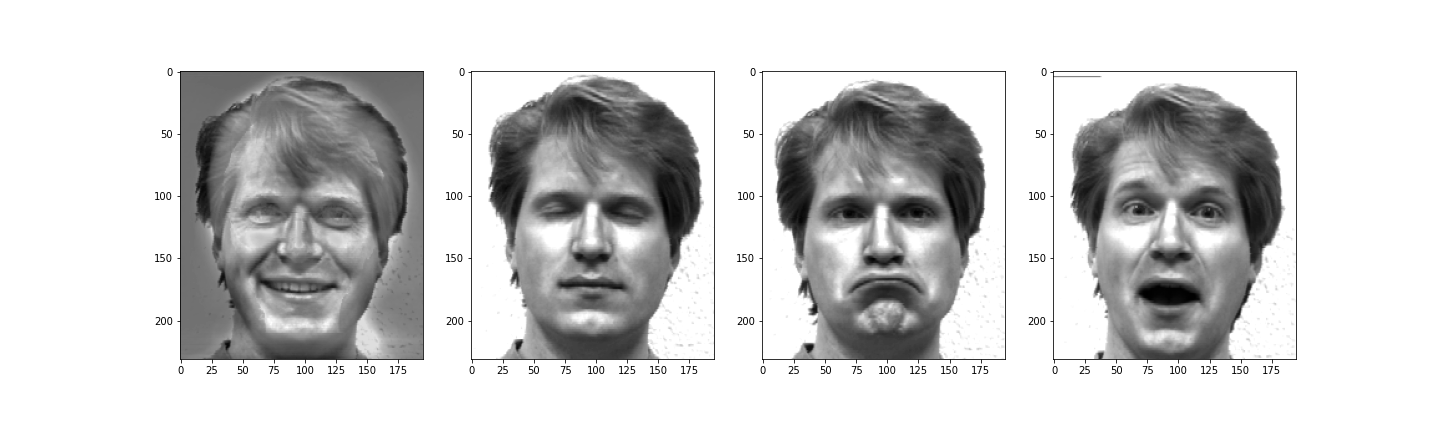
\includegraphics[width=15cm]{2top3.png}
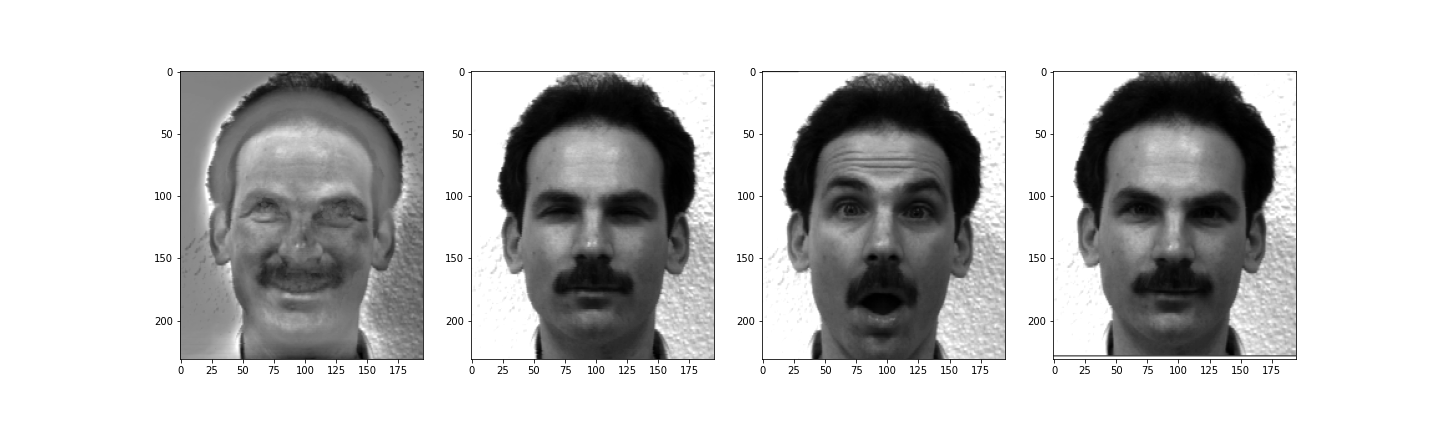
\includegraphics[width=15cm]{3top3.png}
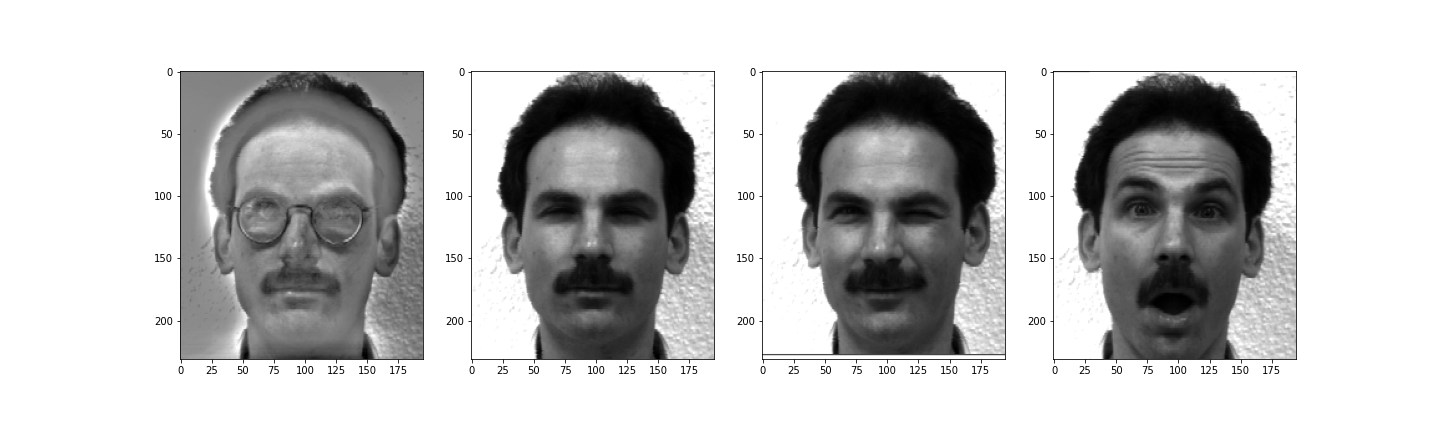
\includegraphics[width=15cm]{4top3.png}
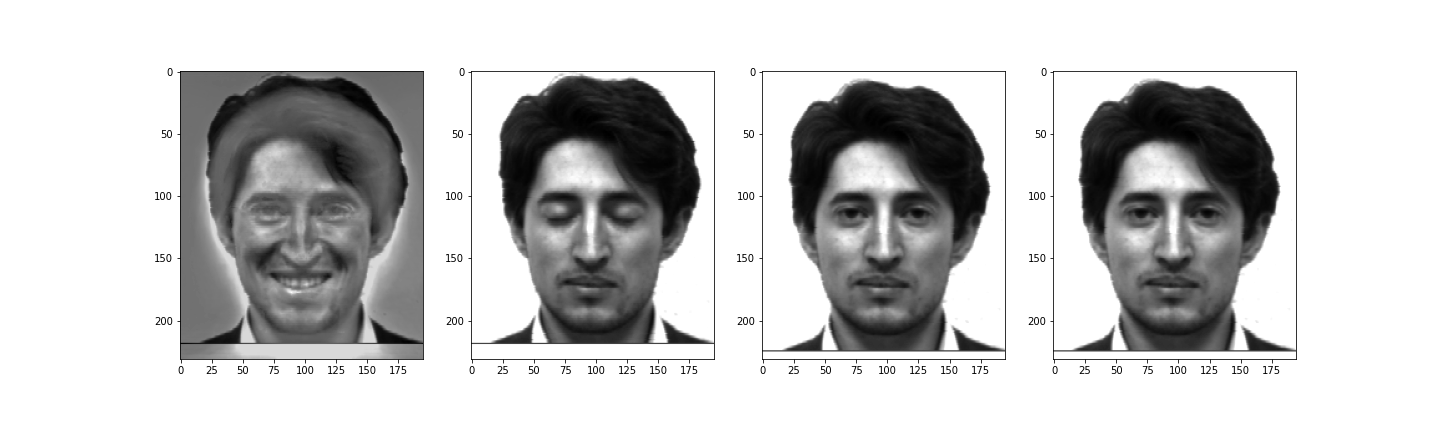
\includegraphics[width=15cm]{5top3.png}
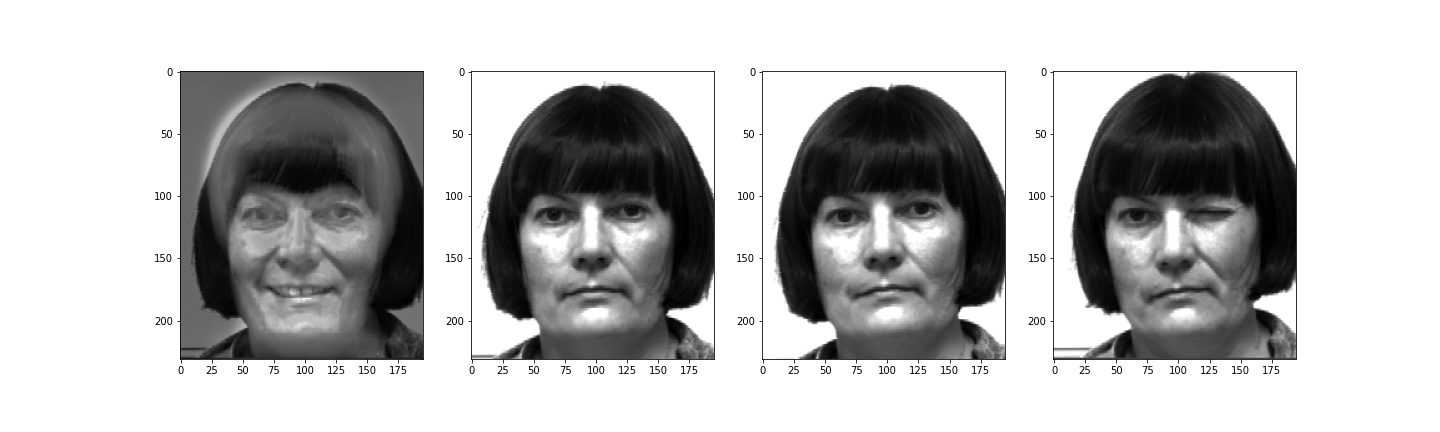
\includegraphics[width=15cm]{6top3.png}
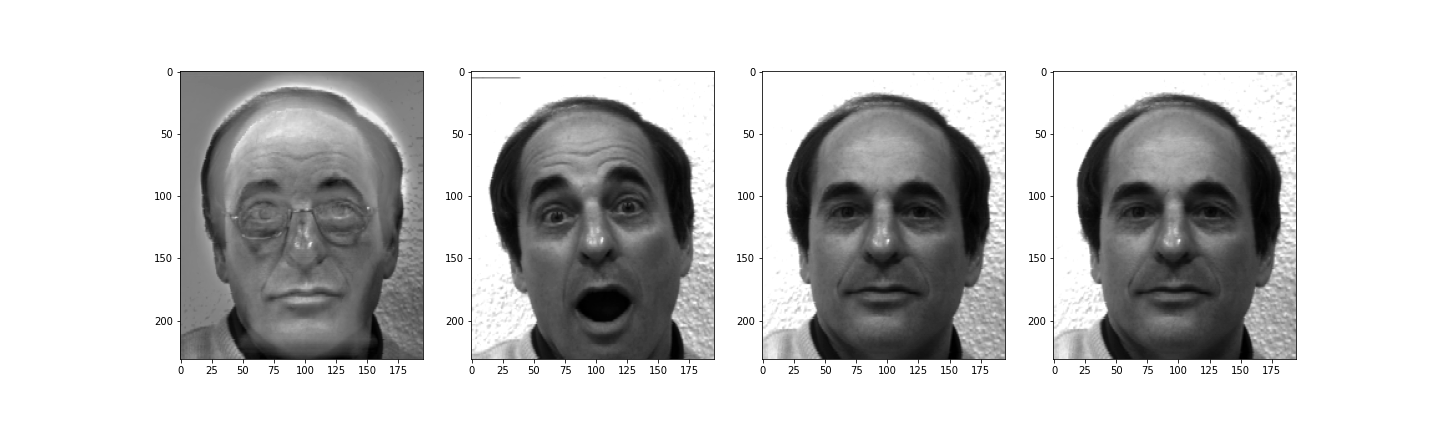
\includegraphics[width=15cm]{7top3.png}
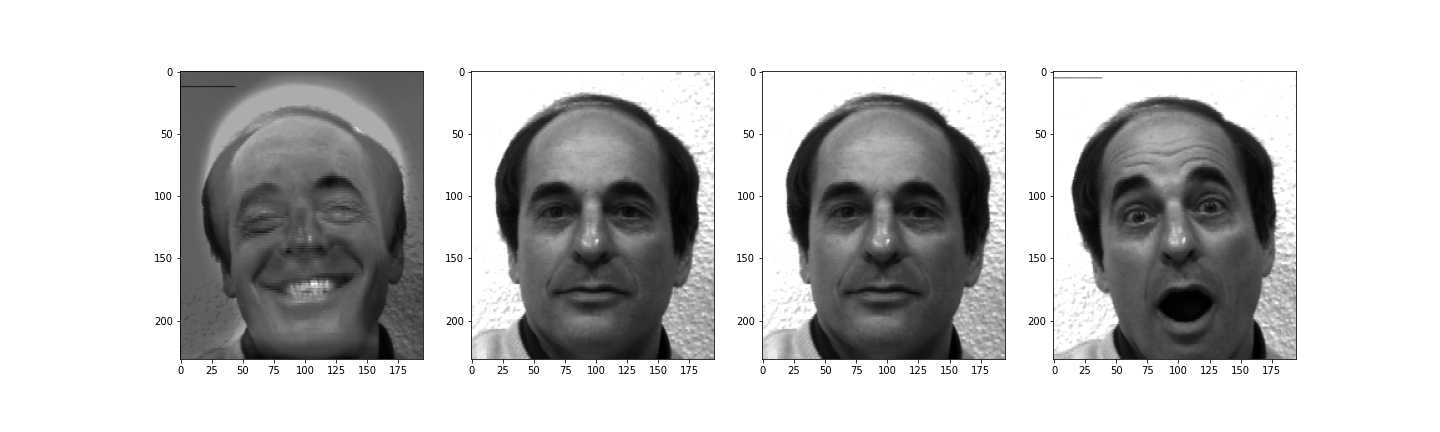
\includegraphics[width=15cm]{8top3.png}
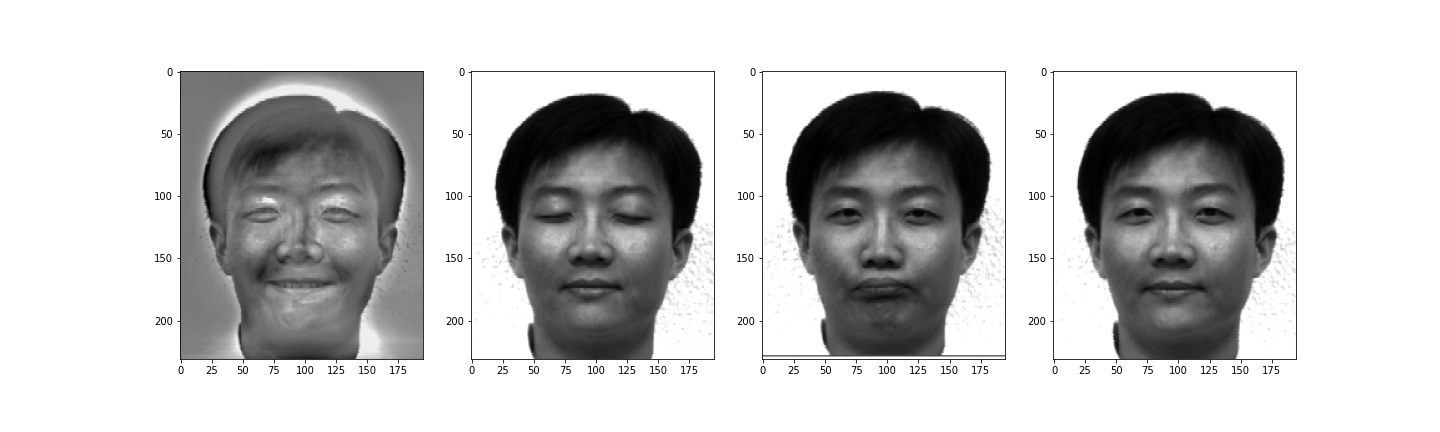
\includegraphics[width=15cm]{9top3.png}
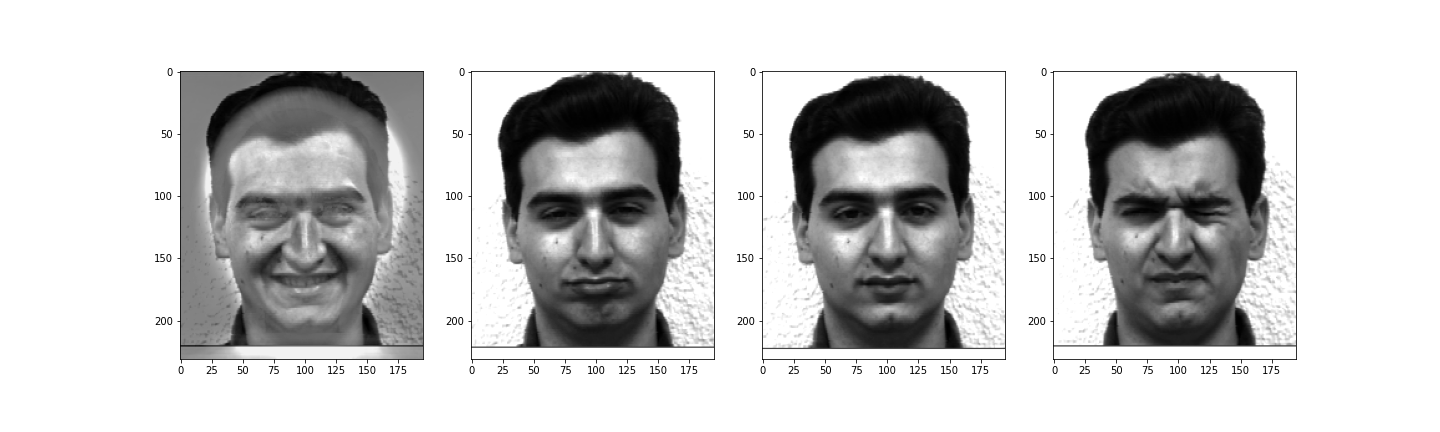
\includegraphics[width=15cm]{10top3.png}

\subsubsection{Read in one of your own frontal face images. Then run your face recognition system on this new image. Display the top 3 faces in the training folder that are most similar to your own face (1 mark).}
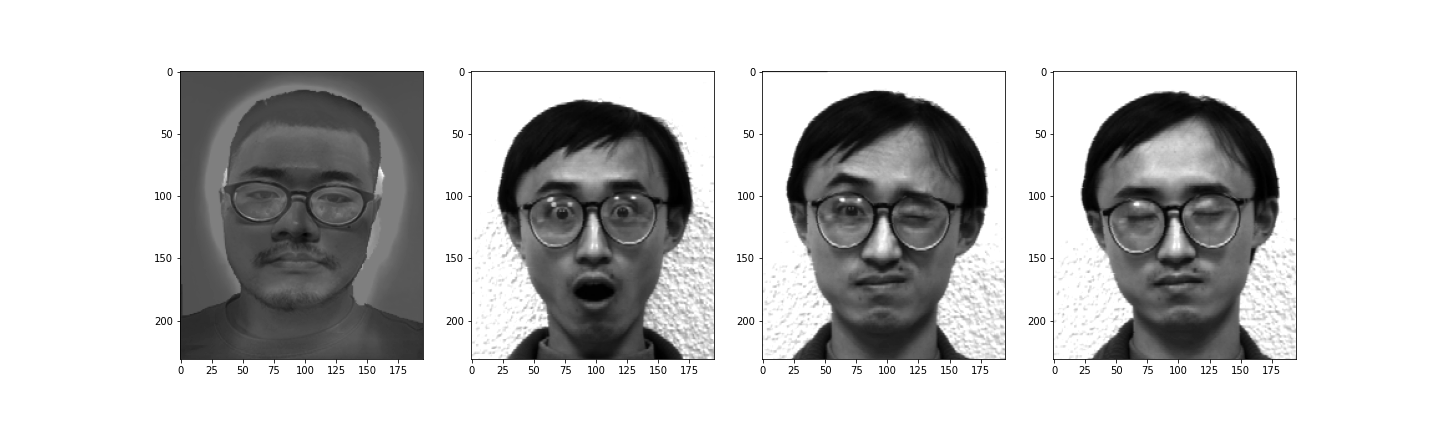
\includegraphics[width=15cm]{mytop3.png}

\subsubsection{Repeat the previous experiment by pre-adding the other 9 additional images of your face into the training set (a total of 144 training images).}
eigenfaces are shown as:\\
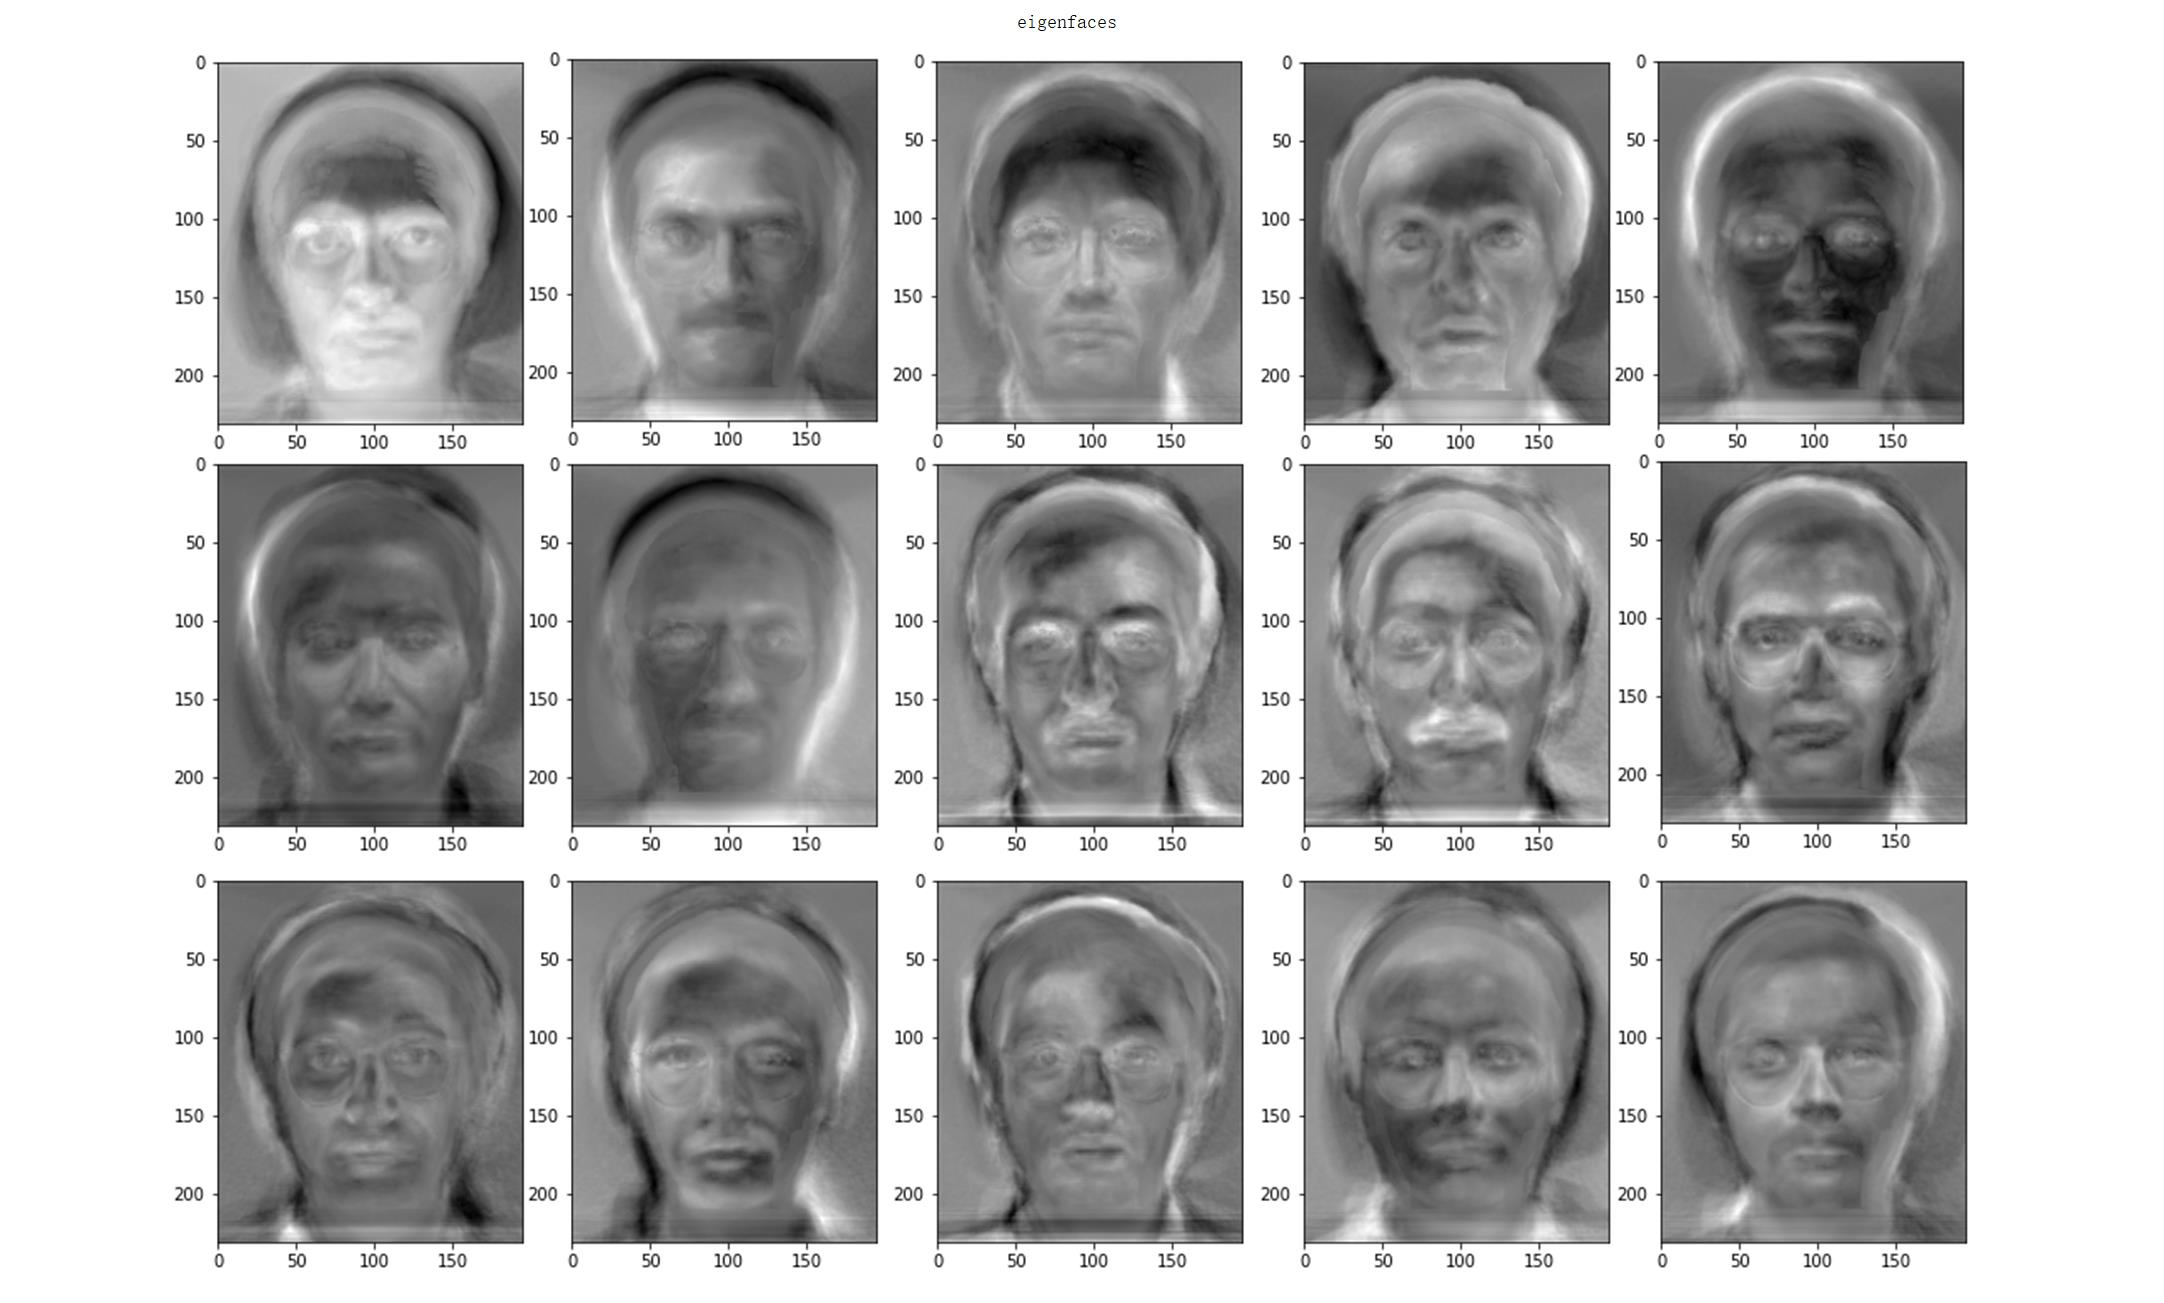
\includegraphics[width=15cm]{eigenfaces2.jpg}\\
Recognization Result and accuracy is 100\%\\
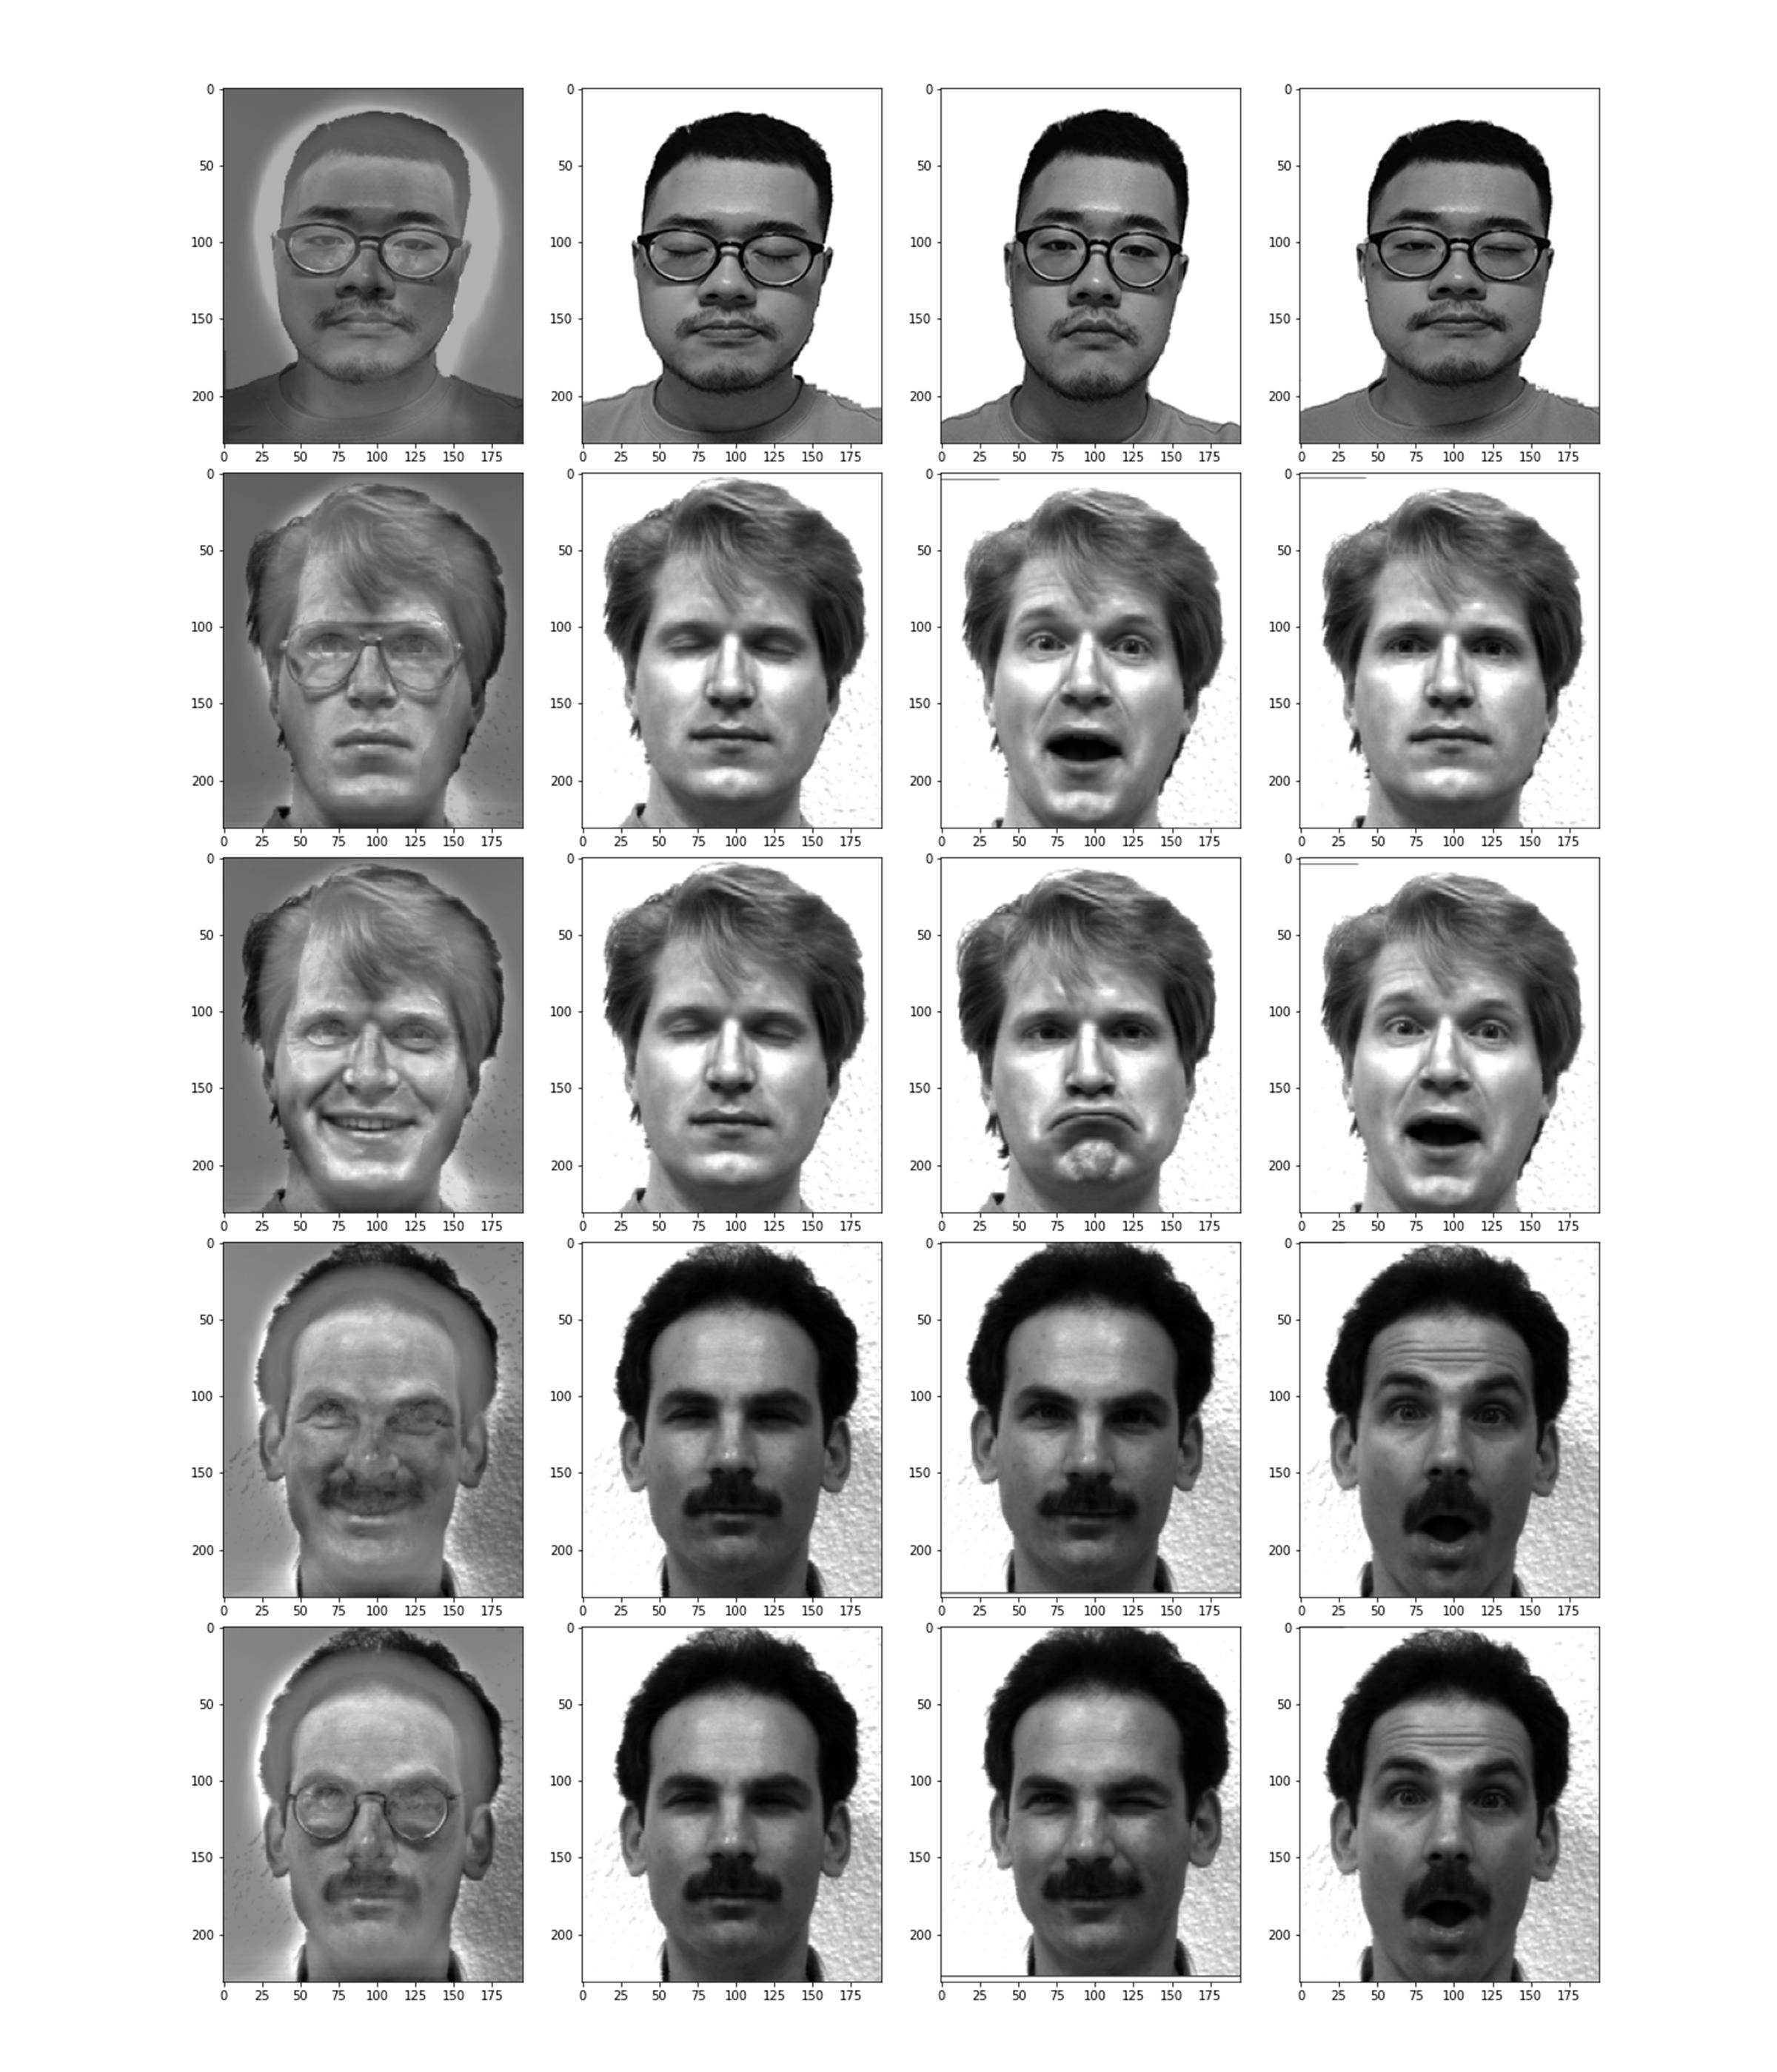
\includegraphics[width=15cm]{result1.jpg}\\
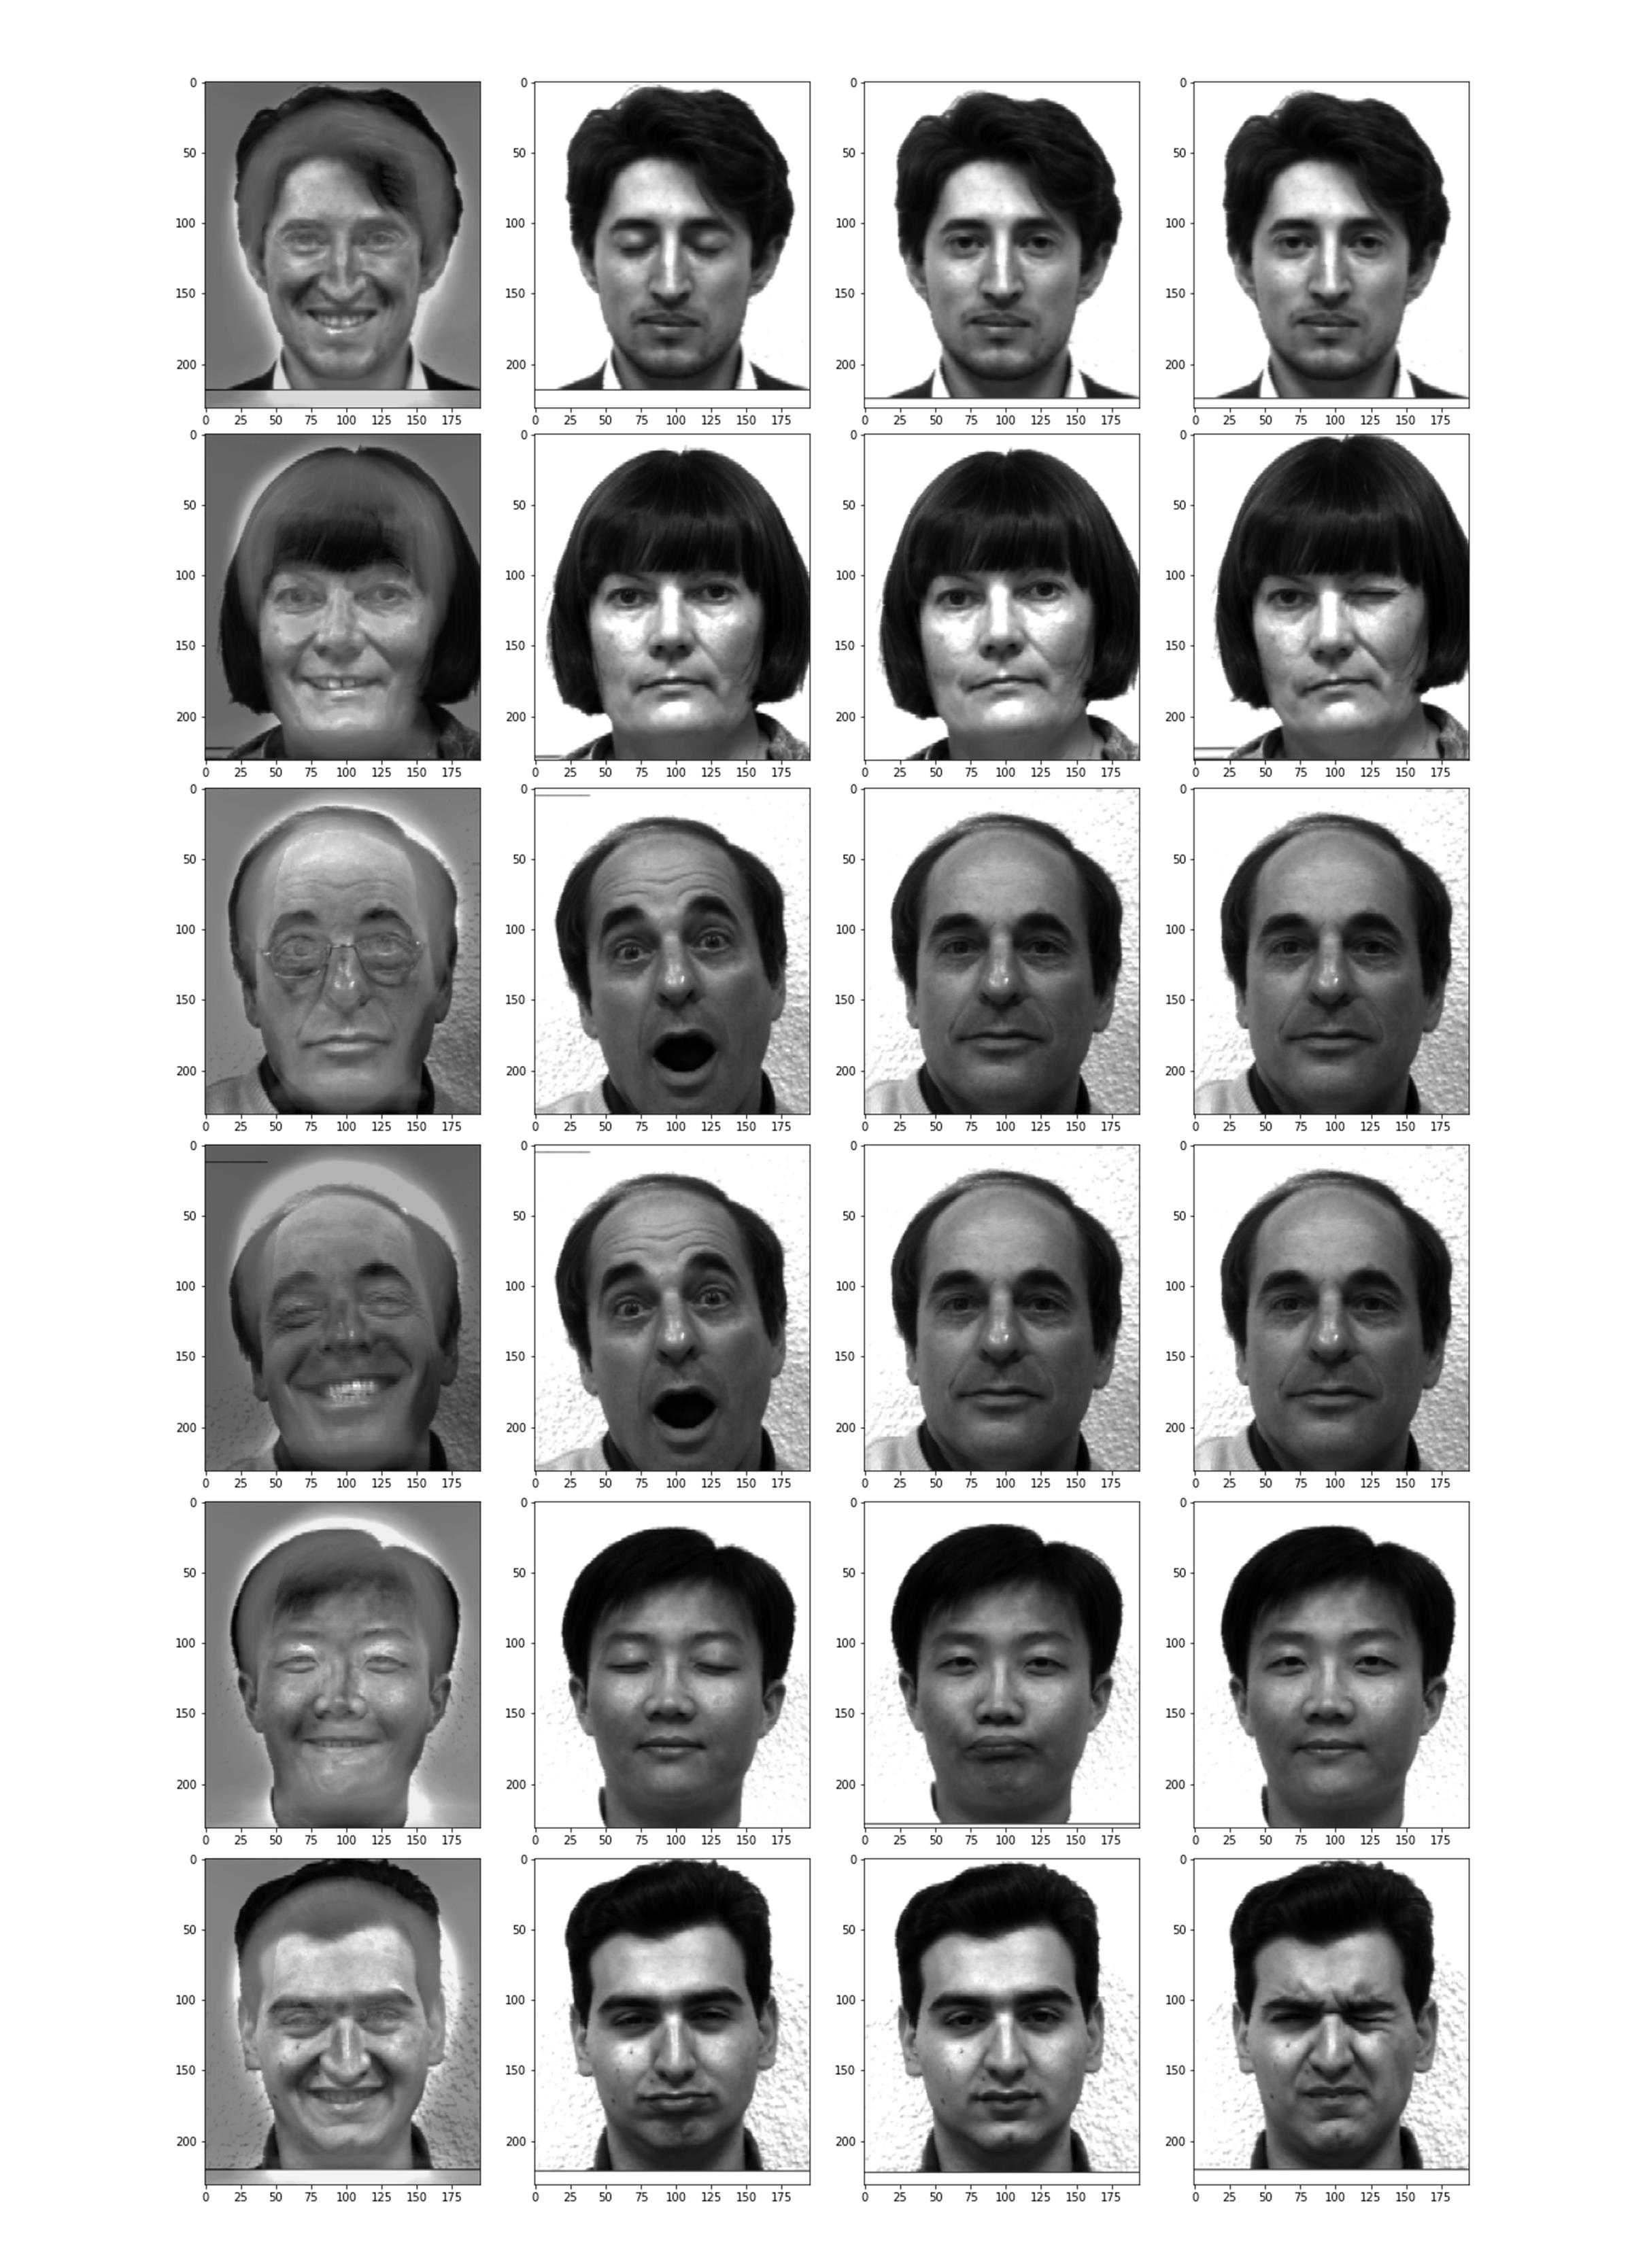
\includegraphics[width=15cm]{result2.jpg}
\end{document}